
%%%%%%%%%%%%%%%%%%%%%%%%%%%%%%%%%%%%%%%%%%%%%%%%%%%%%%%%%%%%%%%%%%%%%%%%%%%%%%%%%%%%%%%%%%%%%%%%%%%%%%%%%%%%
% Author: Omar Portillo
%%%%%%%%%%%%%%%%%%%%%%%%%%%%%%%%%%%%%%%%%%%%%%%%%%%%%%%%%%%%%%%%%%%%%%%%%%%%%%%%%%%%%%%%%%%%%%%%%%%%%%%%%%%%

%Abstract: 0.5
%Intro: 2
%Bg: 2
%Approach/Architecture: 3
%Experiments/Results: 5
%Related Work: 1
%Conclusions: 0.5
%References:  1

%%%%%%%%%%%%%%%%%%%%%%%%%%%%%%%%%%%%%%%%%%%%%%%%%%%%%%%%%%%%%%%%%%%%%%%%%%%%%%%%%%%%%%%%%%%%%%%%%%%%%%%%%%%%
% Defining document class + packages to be used
%%%%%%%%%%%%%%%%%%%%%%%%%%%%%%%%%%%%%%%%%%%%%%%%%%%%%%%%%%%%%%%%%%%%%%%%%%%%%%%%%%%%%%%%%%%%%%%%%%%%%%%%%%%%

\documentclass[runningheads,a4paper]{llncs}

\usepackage{amssymb}
\setcounter{tocdepth}{3}
\usepackage{graphicx}
\usepackage{epstopdf}
\usepackage[linesnumbered,ruled,vlined]{algorithm2e}

\usepackage{url}
\newcommand{\keywords}[1]{\par\addvspace\baselineskip
\noindent\keywordname\enspace\ignorespaces#1}

%Commands needed to define the max size a float can have without been presented
% ALONE in a page.
\renewcommand\topfraction{0.85}
\renewcommand\bottomfraction{0.85}
\renewcommand\textfraction{0.1}
\renewcommand\floatpagefraction{0.85}

%Commands to redice the space before and after floats (like table,fig or alg)
\setlength\floatsep{1.25\baselineskip plus 3pt minus 2pt}
\setlength\textfloatsep{1.25\baselineskip plus 3pt minus 2pt}
\setlength\intextsep{1.25\baselineskip plus 3pt minus 2 pt}

\setlength{\belowcaptionskip}{-7.5pt}
\setlength{\abovecaptionskip}{-2.5pt}

\begin{document}

%%%%%%%%%%%%%%%%%%%%%%%%%%%%%%%%%%%%%%%%%%%%%%%%%%%%%%%%%%%%%%%%%%%%%%%%%%%%%%%%%%%%%%%%%%%%%%%%%%%%%%%%%%%%
% TITLE + AUTHORS' INFORMATION
%%%%%%%%%%%%%%%%%%%%%%%%%%%%%%%%%%%%%%%%%%%%%%%%%%%%%%%%%%%%%%%%%%%%%%%%%%%%%%%%%%%%%%%%%%%%%%%%%%%%%%%%%%%%

\mainmatter  % start of an individual contribution

% first the title is needed
\title{Towards an Automated Approach to Apply the Idle-time Analysis
in Performance Testing}

% a short form should be given in case it is too long for the running head
\titlerunning{Automated Approach to Apply Idle-time Analysis
in Performance Testing}

% the name(s) of the author(s) follow(s) next
%
% NB: Chinese authors should write their first names(s) in front of
% their surnames. This ensures that the names appear correctly in
% the running heads and the author index.
%
\author{A. Omar Portillo-Dominguez\inst{1}\and Miao Wang\inst{1}\and Philip
Perry\inst{1} \and\\
John Murphy\inst{1} \and Nick Mitchell\inst{2}\and Peter F. Sweeney\inst{2}}

\authorrunning{A.O. Portillo-Dominguez et al.}
% (feature abused for this document to repeat the title also on left hand pages)

\urldef{\mailucdconnect}\path|andres.portillo-dominguez@ucdconnect.ie,|
\urldef{\mailucd}\path|{philip.perry,miao.wang,j.murphy}@ucd.ie,|
\urldef{\mailibm}\path|{nickm,pfs}@us.ibm.com|

% the affiliations are given next; don't give your e-mail address
% unless you accept that it will be published
\institute{Lero - The Irish Software Engineering Research Centre, Performance\\
Engineering Laboratory, UCD School of Computer Science and Informatics,
University College Dublin, Ireland\\
\mailucdconnect\\
\mailucd\\
%\url{http://www.ucd.ie/}
\and
IBM T.J. Watson Research Center,\\
Yorktown Heights, New York, USA\\
\mailibm}%\\
%\url{http://www.ibm.com/}


\toctitle{Lecture Notes in Computer Science}
\tocauthor{Authors' Instructions}
\maketitle

%%%%%%%%%%%%%%%%%%%%%%%%%%%%%%%%%%%%%%%%%%%%%%%%%%%%%%%%%%%%%%%%%%%%%%%%%%%%%%%%%%%%%%%%%%%%%%%%%%%%%%%%%%%%
% Abstract 
%%%%%%%%%%%%%%%%%%%%%%%%%%%%%%%%%%%%%%%%%%%%%%%%%%%%%%%%%%%%%%%%%%%%%%%%%%%%%%%%%%%%%%%%%%%%%%%%%%%%%%%%%%%%
\vspace{-15pt}
\begin{abstract}
Performance testing in highly distributed environments is a very challenging
task. Specifically, the identification of performance issues and
the diagnosis of their root causes are time-consuming and complex
activities which usually require multiple tools and heavily rely on the
expertise of the engineers. WAIT, a tool that implements the idle-time analysis,
has proven successful in simplifying the identification of performance issues
and their root causes, hence reducing the dependency to expert knowledge and 
increasing the productivity. However WAIT has some usability limitations that
prevent its efficient usage in performance testing. This paper presents an 
light-weight approach that addresses those limitations and automate WAIT's
usage, making it useful in performance testing. This work was validated through
two case studies with real-life applications, assessing the approach in terms of
overhead costs and time savings in the analysis of performance issues.
The current results have proven the benefits of the approach by achieving a good
decrement in the time invested in performance analysis while only generating a low 
overhead in the tested system.
\vspace{-2pt}
\keywords{Performance testing, automation, performance analysis, idle-time
analysis, distributed environments, multi-tier applications}
\end{abstract}
\vspace{-22pt}
%%%%%%%%%%%%%%%%%%%%%%%%%%%%%%%%%%%%%%%%%%%%%%%%%%%%%%%%%%%%%%%%%%%%%%%%%%%%%%%%%%%%%%%%%%%%%%%%%%%%%%%%%%%%
% Introduction
%%%%%%%%%%%%%%%%%%%%%%%%%%%%%%%%%%%%%%%%%%%%%%%%%%%%%%%%%%%%%%%%%%%%%%%%%%%%%%%%%%%%%%%%%%%%%%%%%%%%%%%%%%%%
\vspace{-2pt}
\section{Introduction}
\vspace{-5pt}
Quality plays a major role in the successful adoption of any software.
Moreover it has a direct impact in the total cost of ownership. For
example, a 2008 Quality Assurance study \cite{CapersJones1} documented that achieving high
quality generates cost savings of around 40\%. It is also an accepted fact that
performance is a critical dimension of quality and should be a major concern of
any software project. This is especially true at enterprise-level, where
performance plays a central role in usability. However it is not uncommon that
performance issues occur and materialize into serious problems (i.e. outages on
production environments, or even cancellation of projects) in a significant
percentage of projects. For example, a 2007 survey applied to
information technology executives \cite{Compuware1} reported that 50\% of them
had faced performance problems in at least 20\% of their deployed applications.

This situation is partially explained by the pervasive nature of
performance, which makes it hard to assess because performance is practically
influenced by every single aspect of the design, code, and execution environment
of an application. Latest trends in the information technology world (such as
Service Oriented Architecture and Cloud Computing) have also augmented the
complexity of applications further complicating activities related to
performance. Under these conditions, it is not surprising that doing performance
testing is complex and time-consuming. A special challenge, documented by
multiple authors \cite{Woodside2007,trevor1,Angelopoulos2012}, is that current
performance tools heavily rely on expert knowledge to understand their output.
It is also common that multiple sources are required to diagnose
performance problems, especially in highly distributed environments. For
instance, in Java thread dumps, garbage collection logs, heap dumps, CPU
utilization and JVM memory usage are a few examples of the information that a
tester could need to understand the performance of an application. This
situation increases the expertise required to do performance analysis, which is
usually held by only a small number of testers within an organization. This
could potentially lead to bottlenecks where some activities can only be done by
experts, hence impacting the productivity of large testing teams.

In addition to the previous challenges, the overhead generated by any technique
should be low to minimize the impact its usage has in the tested environment in
terms of response time and throughput, otherwise the technique would not be
suitable for performance testing. Similarly, if a tool requires heavy human
effort to be used, this might limit the applicability of that tool. On the
contrary, automation could play a key role to encourage the adoption of a
technique. As documented by the authors of \cite{Shahamiri1}, this strategy has
proven successful in perform testing activities.

To ensure that our research work is helpful for solving real-life problems in
the software industry, we have also carried out regular meetings with the IBM
System Verification Test (SVT) to discuss the challenges that they experience in
their day-to-day testing activities. The received feedback confirms that there
is a real need to have tools that can help to improve the performance of the
testing teams by allowing testers with less expertise to carry out analysis
tasks in less time.

WAIT \footnote{http://wait.ibm.com} (an expert system that performs idle-time
analysis) has proven successful in simplifying the detection of performance
issues and their root causes in Java environments \cite{Altman2010,Wu1}.
WAIT is an attractive candidate to the performance testing domain because it has
minimal impact in the monitored environment by using a light-weight monitoring
approach that does not require instrumentation. However WAIT has usability
limitations that prevent its effective usage in performance testing: The overall
data collection process needs to be controlled manually, which in a highly
distributed environment (composed of multiple nodes to monitor and coordinate
simultaneously) would be very time-consuming and error-prone, especially if the
data needs to be refreshed periodically during the test execution to have an
incremental view of the results. This is highly desirable in long runs (i.e. 5
days or more) so that a tester does not need to wait until the end of a test run
to know if any performance issues exist. Even though these limitations might be
manageable in small testing environments, they prevent WAIT to be effectively
use in bigger testing environments as the time and effort required to
synchronize WAIT execution and analyze its outputs would overcome the possible
benefits of its usage. As a highly distributed environment is precisely the
scenario where WAIT's analysis capabilities would be more valuable to simplify
the identification and diagnosis of performance issues, these usage limitations
must be addressed.

This paper proposes a lightweight automated approach that addresses the above
limitations to use WAIT effectively in the performance testing domain, keeping
WAIT's strengths of low overhead and minimal intrusion. This work was achieved
through a two-phase experiment using two real-world applications. The first
phase concentrated in validating that the overhead remained low. The second
phase assessed the productivity benefits that an automated WAIT bring to the
performance testing process. The current results have provided evidence about
the benefits of the approach: The overhead in the monitored system was low
(between 0\% to 3\% when using a common industry \emph{Sample Interval}).
Regarding time savings, using the automated approach added practically no extra
effort to the tester and the time required by a tester to analyze WAIT's outputs
was reduced. Now a tester only needs to review a single WAIT report instead of
multiple individual reports on a node basis. Moreover the consolidated WAIT
report allowed to quickly identify the presence of performance issues, also
pinpointing the responsible classes and method calls. In conclusion, the main
contribution of this paper is a lightweight approach to automate the data
gathering and execution of WAIT in sync with a performance test loader to make
WAIT usable in performance testing.

The rest of this paper is structured as follows: Section 2 discusses the
background. Section 3 shows the related work. Section 4 summarizes the
problem definition. Section 5 describes the proposed approach, while Section 6
explores the experimental evaluation and results. Finally Section 7 presents the
conclusions and future work.

%%%%%%%%%%%%%%%%%%%%%%%%%%%%%%%%%%%%%%%%%%%%%%%%%%%%%%%%%%%%%%%%%%%%%%%%%%%%%%%%%%%%%%%%%%%%%%%%%%%%%%%%%%%%
% Background
%%%%%%%%%%%%%%%%%%%%%%%%%%%%%%%%%%%%%%%%%%%%%%%%%%%%%%%%%%%%%%%%%%%%%%%%%%%%%%%%%%%%%%%%%%%%%%%%%%%%%%%%%%%%
\vspace{-5pt}
\section{Background}
\vspace{-5pt}
\emph{Idle-time analysis} is an analysis methodology that pursues to
explain the root causes that lead to under-utilized resources. This approach,
proposed by \cite{Altman2010}, is based on the observed behavior that in
multi-tier applications performance problems usually manifest as idle time
indicating a lack of forward motion.  WAIT is a tool that implements the
idle-time analysis and identifies the main performance inhibitors that exist on
a system. WAIT is based on non-intrusive sampling mechanisms available at
Operating System level (i.e. ``ps'' and ``vmstat'' commands in a Unix/Linux
environment) and the Java Virtual Machine (JVM), in the form of \emph{Javacores} \footnote{http://www-01.ibm.com/support/docview.wss?uid=swg27017906\&aid=1} 
(diagnostic feature of Java to get a quick snapshot of the JVM state, offering
information such as threads, locks and memory). The fact that WAIT uses standard
data sources makes it non-disruptive, as no special flags or instrumentation are
required to use it. Moreover WAIT requires infrequent samples to perform its
diagnosis, so it also has low overhead. 

From a usability perspective, WAIT is simple: A user only needs to collect as
much data as desired, upload it to a web page and obtain a report with the
findings. Internally, WAIT uses an engine built on top of a set of expert rules
that perform the analysis. \figurename ~\ref{fig_WAITReport} shows an example of
a WAIT Report. The top area summarizes the usage of resources (i.e. CPU, thread
pools and Java Heap) and the number and type of threads per sample. The bottom
section shows all the performance inhibitors that have been identified, ranking
them by frequency and impact. For example, in \figurename ~\ref{fig_WAITReport}
the top issue appeared in 53\% of the samples and affected 7.6 threads on
average. The affected resource was the network and was caused by database readings.

\vspace{-5pt}
\begin{figure}[!h]
\centering
\includegraphics[totalheight=.25\textheight,width=0.9\textwidth]{1exampleReport}
\caption{Example of WAIT Report}
\label{fig_WAITReport}
\end{figure}

%%%%%%%%%%%%%%%%%%%%%%%%%%%%%%%%%%%%%%%%%%%%%%%%%%%%%%%%%%%%%%%%%%%%%%%%%%%%%%%%%%%%%%%%%%%%%%%%%%%%%%%%%%%%
% Related Work
%%%%%%%%%%%%%%%%%%%%%%%%%%%%%%%%%%%%%%%%%%%%%%%%%%%%%%%%%%%%%%%%%%%%%%%%%%%%%%%%%%%%%%%%%%%%%%%%%%%%%%%%%%%%
\vspace{-10pt}
\section{Related Work}
\vspace{-5pt}
The idea of applying automation in the performance testing domain is not new.
However, most of the research has focused on automating the generation of load
test suites
\cite{Chen1,Elvira1,Zhang1,Briand1,Bayan1,Avritzer2,Avritzer3,Garousi1}.
Regarding the performance analysis, a high percentage of the proposed
techniques require instrumentation. For example, the authors of \cite{Yang1}
instrument the source code to mine the sequences of call graphs to infer any
relevant error patterns. A similar case occurs with the work presented in
\cite{Hangal1,Csallner1} which rely on instrumentation to dynamically inferred
invariants and detect programming errors; or the approach proposed by
\cite{Chen2} which uses instrumentation to capture execution paths to determine
the distributions of normal paths and look for any significant deviations to
detect errors. In all cases, instrumentation would obscure the performance of an
application during performance testing hence discouraging their usage. On the
contrary, our proposed approach does not require instrumentation.

One of the closest works to ours is \cite{Jiang2009}. Here the authors present a
non-intrusive approach which automatically analyzes the execution logs of a load
test to identify performance problems. As this approach only analyzes load
testing results, it can not determine root causes. The other work which is
closest to ours is \cite{Malik1} which pursues to offer information about the
causes behind the issues. However it can only determine the subsystem
responsible of the performance deviation. In both cases, the techniques also
require information from previous runs as baseline to do their analysis,
information which might not always be available. Finally, to the best of our
knowledge, our approach is the first to propose the applicability through
automation means of the idle-time analysis in the performance testing domain to
exploit its performance analysis capabilities.

%%%%%%%%%%%%%%%%%%%%%%%%%%%%%%%%%%%%%%%%%%%%%%%%%%%%%%%%%%%%%%%%%%%%%%%%%%%%%%%%%%%%%%%%%%%%%%%%%%%%%%%%%%%%
% Problem Definition
%%%%%%%%%%%%%%%%%%%%%%%%%%%%%%%%%%%%%%%%%%%%%%%%%%%%%%%%%%%%%%%%%%%%%%%%%%%%%%%%%%%%%%%%%%%%%%%%%%%%%%%%%%%%
\vspace{-5pt}
\section{Problem Definition}
\vspace{-5pt}
While doing performance testing in highly distributed environments, the
identification of performance problems and the diagnosis of their root causes
are very complex and time-consuming activities, which tend to rely on the
expertise of the involved engineers. Due to its strengths, WAIT is a promising
candidate to improve this scenario by reducing the expert knowledge and time
required to do performance analysis. However, WAIT has some usability
limitations that prevent its effective usage in performance testing: The effort
required to do manual data collection to feed WAIT and the number of WAIT
reports a tester would need to review are practically lineal with respect of the
number of application nodes and the frequency with which the data needs to be
refreshed. For example, assuming a relatively small environment composed of 10
application nodes, a 24-hour test run and a refresh frequency of 1 hour, a
tester would need to coordinate 10 simultaneous data collection and upload
cycles per hour (for a total of 240 cycles), doing them as fast as possible to
minimize the time gaps between the end of a cycle and the start of the next.
Additionally, the tester should review the 10 different WAIT reports he would
get every hour, and compare them with the previous ones, to see if there are
any performance issues. As it can be inferred from this example, the current
cost of using WAIT in a highly distributed environment would overcome the
benefits, as it would be a very effort-intensive and error-prone process.

The objective of this paper is to address the usability limitations of WAIT to
be used effectively in performance testing. To achieve this, the following
research questions have been formulated:
\\Q1. How can the usage of WAIT be automated to minimize the effort
required to use it in sync with a performance test?
\\Q2. Can the overhead be kept low during a performance test execution to avoid
compromising the results?
\\Q3. What benefits in productivity can a tester achieve if the previous
two questions are answered?

The following sections show how these questions were answered by our approach
and validated through a series of experiments.

%%%%%%%%%%%%%%%%%%%%%%%%%%%%%%%%%%%%%%%%%%%%%%%%%%%%%%%%%%%%%%%%%%%%%%%%%%%%%%%%%%%%%%%%%%%%%%%%%%%%%%%%%%%%
% Proposed Approach
%%%%%%%%%%%%%%%%%%%%%%%%%%%%%%%%%%%%%%%%%%%%%%%%%%%%%%%%%%%%%%%%%%%%%%%%%%%%%%%%%%%%%%%%%%%%%%%%%%%%%%%%%%%%
\vspace{-5pt}
\section{Proposed Approach and Implementation}
\vspace{-5pt}
%This section presents the details of the proposed approach, its architecture
%and the prototype that has been developed to validate it.

Our approach is depicted in the Algorithm~\ref{Proposed_Approach} and requires
a few inputs: The list of nodes that will be monitored (usually all the nodes
that composed the tested system); a \emph{Sampling Interval} to control how
often the samples will be collected; a \emph{Time Threshold} which indicates the
maximum time without refreshing the results; a \emph{Hard Disk Threshold} which
indicates the maximum space to store collected data per node; and a
\emph{Backup} flag that indicates if the collected data should be backed up
before any cleaning occurs.

\begin{algorithm}
\caption{Proposed Approach}
\label{Proposed_Approach}
\DontPrintSemicolon
\KwIn{ A finite set $A=\{a_1, a_2, \ldots, a_n\}$ of application nodes, 
Sampling Interval \emph{Sint}, Time Threshold \emph{tThres}, Hard Disk Threshold
\emph{hdThres}, Backup Flag \emph{bFlag}. 
If \emph{bFlag} = true, Backup path \emph{bPath}.}
\KwOut{Incremental WAIT report for all Nodes}
\tcp*[h]{Initialization}\;
$rundId \gets $new RunId\;
share $rundId$ \hspace{2 mm} with all nodes\;
\For{$i \gets 1$ \textbf{to} $n$ nodes} {	
	$hdUsage \gets 0$\;
	$nextTimeThreshold \gets $current time from the Operating System + $tThres$\;
			
    \tcp*[h]{Main Process}\;
	\While{Performance Testing is executing}{
		\tcp*[h]{Data gathering}\;
		Collect new set of samples (process and machine utilization as well
	    as a new javacore per JVM process in the node)\;
		\tcp*[h]{Refresh performance results}\;
		$currentTime \gets $current time from the Operating System\;
		$hdCurrentUsage \gets $calculate Hard Disk space of collected data\;
		\If{$currentTime$ $>$ $nextTimeThreshold$ or $hdCurrentUsage$ $>$ $hdThres$} {
			update locally collected data indicating it as part of test $rundId$\;
			\If{$bFlag$ $=$ true} {
				copy locally collected data to $bPath$ indicating it as part of test
				$rundId$\;
			}
			deleted locally collected data\;
			retrieve updated performance results\;
			$nextTimeThreshold \gets $current time from the Operating System + $tThres$\; 
			}
	    Wait $Sint$ before performing next iteration of the process\;
	}
	
	\tcp*[h]{Closure}\;
	update remnant locally collected data indicating it as part of test $rundId$\;
	\If{$bFlag$ $=$ true} {
		copy remnant locally collected data to $bPath$ indicating it as part of test
		$rundId$\; 
		}
		deleted remnant locally collected data\;
  }
  Retrieve final performance results\;
\end{algorithm}

The process starts by getting a new \emph{RunId}, value which will uniquely
identify the test run and its results. This value is propagated to all
the nodes. On each node, the \emph{Hard Disk Usage} and  the \emph{Next Time
Threshold} are initialized. Then each node starts the following
loop until the performance test finishes: A new set of data samples is
collected (composed of machine and process utilization and a \emph{Javacore}
from each running JVM). After the collection finishes, it is assessed if any of
the two thresholds has been reached (either the \emph{Hard Disk Usage} has
exceeded the \emph{Hard Disk Threshold} or the \emph{Next Time Threshold} has
been reached). If any of the conditions has occurred, a new upload round occurs
where the data is uploaded to the WAIT server (labeling the data with the
\emph{RunId} so that uploads of different nodes are identified as part of the
same test run). If a \emph{Backup} was enabled, the data is copied to the backup
destination before it is deleted. Then a reference to the updated WAIT report is
obtained and the \emph{Next Time Threshold} is calculated. Finally, the logic
awaits the configured \emph{Sampling Interval} before a new iteration starts.

Once the performance test finishes, a final upload round (and backup if
configured) is done to upload any remnant collected data. When completed this
data is also cleared and the \textbf{final performance results report} is
obtained.

To achieve a lightweight automation, the previous approach was complemented with
the architecture presented in the \figurename ~\ref{fig_Arch}. It is composed of
two main components. The \emph{WAIT Control Agent} which is responsible of
interacting with the Load Testing tool to know when the performance test starts
and ends. Also it is responsible of getting the runId and propagate it to all
the nodes. The second component is the \emph{WAIT Node Agent} which
is responsible of the collection, upload, backup and cleanup steps in each
application node.

Based on the concepts presented here, a prototype has been developed in
conjunction with our industrial partner IBM. The \emph{WAIT Control Agent} was
implemented as a Eclipse Plugin for the Rational Performance Tester (RPT)
\footnote{http://www-03.ibm.com/software/products/us/en/performance},
while the \emph{WAIT Control Agent} was implemented as a Java Web Application.
In both cases, the involved technologies (Eclipse Plugin and Web Application)
were selected because they are simply to install. Once installed, WAIT can now
be configured as any other resource in RPT. This is shown in \figurename
~\ref{fig_config}. Similarly, during a performance test WAIT can be monitored as
any other resource in the \emph{Performance Report} of RPT under the
\emph{Resource View}. This is shown in the \figurename ~\ref{fig_mon}. Finally,
the incremental WAIT report is also accessible within RPT, so a tester does not
need to leave RPT during the whole duration of the performance test. This is
shown in \figurename ~\ref{fig_report}.

\vspace{-5pt}
\begin{figure}[!h]
\centering
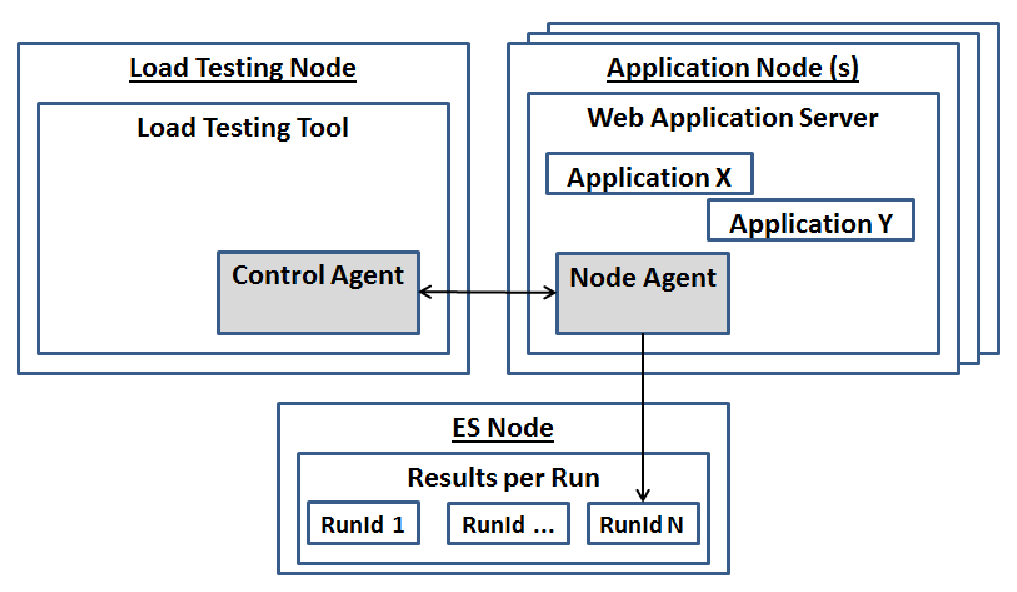
\includegraphics[totalheight=.3\textheight,width=0.9\textwidth]{architecture_dwait}
\caption{High-level Architecture of the solution}
\label{fig_Arch}
\end{figure}
\vspace{-5pt}

\vspace{-5pt}
\begin{figure*}
\centering
\begin{minipage}[b]{.45\textwidth}

\centering
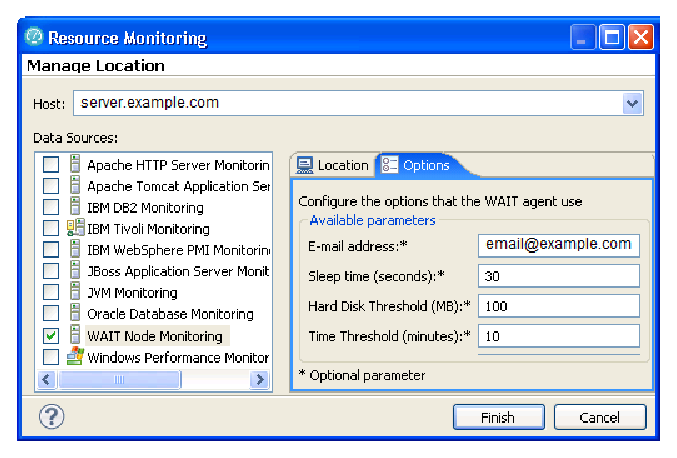
\includegraphics[totalheight=.3\textheight,width=1.0\textwidth]{WAIT-config}
\caption{WAIT configuration in RPT}
\label{fig_config}

\end{minipage}\qquad
\begin{minipage}[b]{.45\textwidth}

\centering
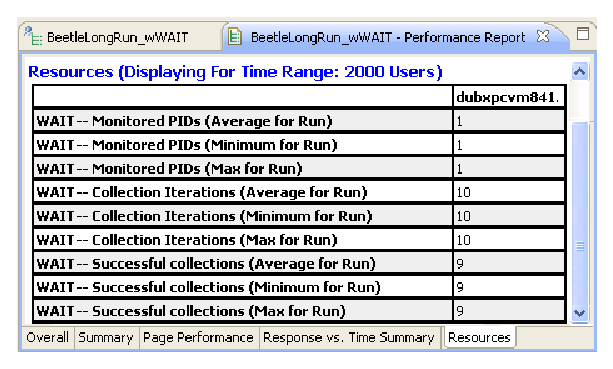
\includegraphics[totalheight=.3\textheight,width=1.0\textwidth]{WAIT-monitoring}
\caption{WAIT monitoring in RPT}
\label{fig_mon}

\end{minipage}
\end{figure*}
\vspace{-5pt}

\vspace{-5pt}
\begin{figure}[!h]
\centering
\includegraphics[totalheight=.35\textheight,width=0.9\textwidth]{WAIT-report}
\caption{WAIT Report accessible in RPT}
\label{fig_report}
\end{figure}

%%%%%%%%%%%%%%%%%%%%%%%%%%%%%%%%%%%%%%%%%%%%%%%%%%%%%%%%%%%%%%%%%%%%%%%%%%%%%%%%%%%%%%%%%%%%%%%%%%%%%%%%%%%%
% Experimental Setup / Experiments
%%%%%%%%%%%%%%%%%%%%%%%%%%%%%%%%%%%%%%%%%%%%%%%%%%%%%%%%%%%%%%%%%%%%%%%%%%%%%%%%%%%%%%%%%%%%%%%%%%%%%%%%%%%%
\vspace{5pt}
\section{Experimental Evaluation and Results}
\vspace{-5pt}
%In this section the experimental setup is presented along with the experiments
% themselves.
%After each experiment, its results are also discussed.

Two experiments were performed. The first one pursed to answer the
research question Q2 (Can the overhead be kept low during a performance test
execution to avoid compromising the results?), while the second one pursued to
answer the research question Q3 (What benefits in productivity can a tester achieve if the previous
two questions are answered?). The combined outcome of the experiments pursued to
answer the research question Q1 (How can the usage of WAIT be automated to
minimize the effort required to use it in sync with a performance test?).

Moreover two environments were used: One was composed of one RPT node,
one application node and one WAIT Server node; the other was composed of one RPT
node, one load balance node, two application nodes and one WAIT Server node. All
nodes were connected by a 10-GBit LAN. These set-ups are shown in \figurename
~\ref{fig_env}.

\vspace{-5pt}
\begin{figure}[!h]
\centering
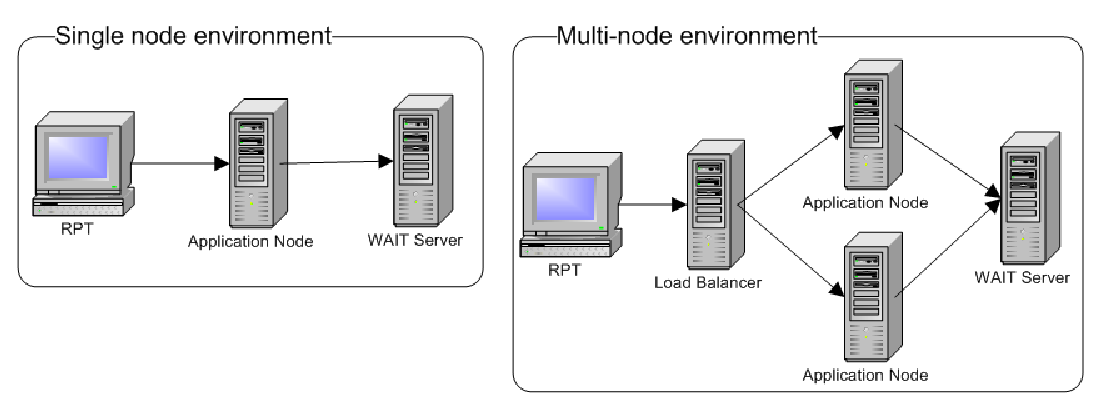
\includegraphics[totalheight=.18\textheight,width=0.8\textwidth]{Environments}
\caption{Environment Set-ups}
\label{fig_env}
\end{figure}

The RPT node ran over Windows XP with an Intel Xeon CPU at
2.67 Ghz and 3GB of RAM using RPT 8.2.1.3. The WAIT Server was ran over Red Hat
Enterprise Linux Server 5.9, with an Intel Xeon CPU at 2.66 GHz and 2GB of
RAM using Apache Web Server 2.2.3. Each application node was a 64-bit Windows
Server 2008, with an Intel Xeon E7-8860 CPU at 2.26 GHz and 4GB of RAM
running Java 1.6.0 IBM J9 VM (build 2.6). Finally, the load balance node had the
same characteristics of the WAIT Server node and used mod\_jk for load balance.
\vspace{-5pt}
\subsection{Experiment \#1}
\vspace{-2pt}
Its objective was to validate that the proposed approach had low overhead and
involved the assessment of four metrics: Throughput, response time, CPU
and memory utilization. All metrics were collected through RPT.
Furthermore 2 real-world applications were used: iBatis JPetStore 4.0
\footnote{http://sourceforge.net/projects/ibatisjpetstore/} which is an upgraded
version of Sun's Pet Store, an e-commerce shopping cart application. It ran over
an Apache Tomcat 6.0.35 Application Server. The other application was IBM
WebSphere Portal Server 8.0.1 \footnote{http://www-03.ibm.com/software/products/us/en/portalserver},
a leader solution in the enterprise portal market \cite{Gartner2008}. It ran
over an IBM WebSphere Application Server 8.0.0.5.

The experiment involved two tests. First, the overhead of the approach was
tested in a single-node environment. For each application, 3 combinations
of WAIT were run: First the application was executed without WAIT to get a
baseline; then a manual WAIT execution (data collection without upload) was
introduced to measure its overhead. Finally, the automated approach was
introduced to measure its overhead. For each combination which used WAIT, 2
\emph{Sampling Interval} were tested: One value (480 seconds) was suggested by
our industrial partner, while the other (30 seconds) was chosen for been the
minimum recommended \emph{Sampling Interval} for WAIT. All additional
test configuration was suggested by our industrial partner: A workload of 2,000
concurrent users; a duration of 1 hour; a \emph{Hard Disk Threshold} of 100MB;
and a \emph{Time Threshold} of 10 minutes. Each combination (5 per application)
was run 3 times.

For JPetStore, each test run produced around 500,000 transactions. The
results showed that using WAIT with a \emph{Sample Interval} of 480 seconds had
practically no impact in terms of response time and throughput. Furthermore the
difference in resource consumption between the manual and automated approaches
was around 1\%.  This difference was mostly related to the presence of the
WebAgent because the uploaded data was very small in this case (around 200KB
every 10 minutes). When WAIT used a \emph{Sample Interval} of 30 seconds, the
impacts in response time and throughput appeared. Considering the throughput was
similar between approaches, the impact should had been caused by the
\emph{Javacore} generation (step shared between the approaches). In average, the
generation of a \emph{Javacore} took around 1 second. Even though this cost was
neglectable in the higher \emph{Sample Interval}, with 30 seconds the impact was
visible. On the contrary, the difference in response times (2.8\%, around 53
milliseconds) was caused by the upload and backup processes (around 4MB of
data), as the cost of the WebAgent had been previously measured. In terms of
resource consumption, the differences between approaches remained within 1\%.
These results are shown in the \tablename ~\ref{PetStore1} where the first row
shows the baseline and the others the percentage differences of each
tested combination.

\begin{table}[!h]
\caption{PetStore - Results}
\label{PetStore1}
\centering
\begin{tabular}{p{0.2\textwidth}|p{0.16\textwidth}|p{0.16\textwidth}|p{0.15\textwidth}|p{0.13\textwidth}|p{0.16\textwidth}}
\hline
\bfseries WAIT Modality & \bfseries Avg Response Time (ms)& \bfseries Max
Response Time (ms)& \bfseries Avg Throughput (hps)& \bfseries Avg CPU Usage
(\%) & \bfseries Avg Memory Usage (MB)\\
\hline
None (\emph{Baseline}) 	& 1889.6	& 44704.0	& 158.8 	& 36.9 		& 1429\\
Manual, 480s 			& 0.0\% 	& 0.0\%		& 0.0\%		& 1.1\% 	& 3.0\%\\
Automated, 480s 		& 0.0\%		& 0.0\%		& 0.0\% 	& 2.0\% 	& 3.7\%\\
Manual, 30s 			& 1.6\%		& 0.4\%		& -4.0\% 	& 1.47\% 	& 4.1\%\\
Automated, 30s 			& 4.4\%		& 0.5\%		& -3.1\% 	& 2.53\% 	& 4.4\%\\
%\hline
%Automated, 480s (2 nodes)& 0.5\%	& 0.2\%		& -1.4\% 	& 0.85\% 	& 2.3\%\\
\hline
\end{tabular}
\end{table}

For Portal, each test run produced around 400,000 transactions. Even though the
results showed similar trends in terms of having lower overheads using the
\emph{Sampling Interval} of 480 seconds, a few key differences were identified:
First, the impacts in response time and throughput were visible since the
\emph{Sampling Interval} of 480 seconds. Besides, the differences between
\emph{Sampling Intervals} were bigger. As the experiment conditions were the
same, it was assumed that these differences were related to the dissimilar
functionality of the tested applications. This was confirmed after analyzing the
\emph{Javacores} generated by the Portal, which allowed to quantify the
differences in behavior of Portal: The average size of a \emph{Javacore} was
5.5MB (450\% bigger than JPetStore's), its average generation time was 2 sec
(100\% bigger than JPetStore's), with a maximum generation time of 3 sec (100\%
bigger than JPetStore's). The results are shown in the \tablename ~\ref{Portal1}.

\begin{table}[!h]
\caption{Portal - Results}
\label{Portal1}
\centering
\begin{tabular}{p{0.2\textwidth}|p{0.16\textwidth}|p{0.16\textwidth}|p{0.15\textwidth}|p{0.13\textwidth}|p{0.16\textwidth}}
\hline
\bfseries WAIT Modality & \bfseries Avg Response Time (ms)& \bfseries Max
Response Time (ms)& \bfseries Avg Throughput (hps)& \bfseries Avg CPU Usage
(\%) & \bfseries Avg Memory Usage (MB)\\
\hline
None (\emph{Baseline}) 	& 4704.75	& 40435.50	& 98.05 	& 76.73 	& 3171.20\\
Manual, 480s 			& 0.7\% 	& 0.6\%		& -0.1\%	& 1.13\% 	& 2.2\%\\
Automated, 480s 		& 3.4\%		& 1.0\%		& -2.8\% 	& 0.63\% 	& 4.1\%\\
Manual, 30s 			& 14.9\%	& 5.4\%		& -5.7\% 	& 2.97\% 	& 5.3\%\\
Automated, 30s 			& 16.8\%	& 9.1\%		& -5.6\% 	& 2.23\% 	& 6.0\%\\
\hline
\end{tabular}
\end{table}

Due to the small differences among the runs and the variations (presumable
environmental) that were experienced during the experiments, a Paired t-Test
\footnote{http://www.aspfree.com/c/a/braindump/comparing-data-sets-using-statistical-analysis-in-excel/},
using a significant level of p<0.1, was done to evaluate if the differences in
response time and throughput were statistically significant. For JPetStore, the
results showed that the differences were only significant in the average
response time using the \emph{Sample Interval} of 30 seconds, and in the average
throughput using the \emph{Sample Interval} if 30 seconds with the automated
approach. Similar results were obtained from Portal. This analysis reinforced
the conclusion that the overhead was low as well as the observation that the
\emph{Sample Interval} of 480 seconds was preferable. These results are shown in
the \tablename ~\ref{tTest1}.

\begin{table}[!h]
\caption{Paired t-Test Results}
\label{tTest1}
\centering
\begin{tabular}{p{0.2\textwidth}|p{0.2\textwidth}|p{0.2\textwidth}|p{0.2\textwidth}|p{0.2\textwidth}}
\hline
\bfseries Application & \bfseries WAIT Modality & \bfseries Avg Response Time
(ms)& \bfseries Max Response Time (ms)& \bfseries Avg Throughput (hps)\\
\hline
PetStore & 	Manual, 480s 			& 0.470 & 0.143	& 0.206\\
PetStore & 	Automated, 480s 		& 0.342	& 0.297	& 0.472\\
PetStore & 	Manual, 30s 			& 0.089	& 0.241	& 0.154\\
PetStore & 	Automated, 30s 			& 0.019	& 0.334	& 0.078\\
\hline
Portal 	& 	Manual, 480s 			& 0.140 & 0.263	& 0.496\\
Portal 	& 	Automated, 480s 		& 0.040	& 0.189	& 0.131\\
Portal 	& 	Manual, 30s 			& 0.001	& 0.158	& 0.167\\
Portal 	& 	Automated, 30s 			& 0.013	& 0.105	& 0.072\\
\hline
\end{tabular}
\end{table}

A second test was done to validate that the overhead of the proposed approach
remained low when used in a multi-node environment over a longer test run.
JPetStore was used for this test. First it was executed alone to have a
baseline; then the automated WAIT approach was introduced using a \emph{Sampling
Interval} of 480 seconds. The rest of the set-up was identical to the previous
tests except the workload which was doubled to compensate the additional
application node and the test duration which was increased to 24 hours. Even
though the results were slightly different than the single-node run, they proved that
the solution was reliable, as using the automated approach had minimal impact in
terms of response time (0.5\% in the average and 0.2\% in the max) and
throughput (1.4\%). Moreover the consumption of resources behaved similar to the
single-node test (an increment of 0.85\% in CPU and 2.3\% in Memory).
%The detailed results of these experiments are shown in the \tablename
% ~\ref{Portal2}.
The performed paired t-Test also indicated that the differences in response time
and throughput between the test runs were not statistically significant.

%\begin{table}[!h]
%\caption{Multi-node PetStore - results}
%\label{Portal2}
%\centering
%\begin{tabular}{p{0.2\textwidth}|p{0.16\textwidth}|p{0.16\textwidth}|p{0.15\textwidth}|p{0.13\textwidth}|p{0.16\textwidth}}
%\hline
%\bfseries WAIT Modality & \bfseries Avg Response Time (ms)& \bfseries Max
%Response Time (ms)& \bfseries Avg Throughput (hps)& \bfseries Avg CPU Usage
%(\%) & \bfseries Avg Memory Usage (MB)\\
%\hline
%None (\emph{Baseline}) 	& 2669.62	& 47346.10	& 157.68 	& 45.27 	& 1831.10\\
%Automated, 480s 		& 0.5\%		& 0.2\%		& -1.4\% 	& 0.85\% 	& 2.3\%\\
%\hline
%\end{tabular}
%\end{table}

In conclusion, the results of this first experiment showed that the overhead
caused by the automated approach remained low. This answered our research
question Q2 positively, but with a side note: Due to the impact that the
\emph{Sampling Interval} and the application behavior could have in the
overhead, it is important to consider this when using WAIT. In our case, a
\emph{Sampling Interval} of 480 seconds proved efficient in terms of overhead
for the two tested applications.

\vspace{-5pt}
\subsection{Experiment \#2}
\vspace{-2pt}
Here the objective was to assess the benefits the approach brings to a
performance tester. For this experiment the automated approach was used to
monitor a modified version of the iBatis PetStore 4.0 application. The source
code was modified to inject some performance issues to assess how WAIT was able
to identify them and estimate the corresponding time savings in performance
analysis. Three common performance issues were injected: A lock contention bug,
composed by a very heavy calculation within a synchronized block of code; a I/O
latency bug, composed by a very expensive file reading method; and a deadlock
bug, an implementation of the classic ``friends bowing'' deadlock example
\footnote{http://docs.oracle.com/javase/tutorial/essential/concurrency/deadlock.html}.
All other set-up parameters were identical to the multi-node test previously
performed with exception of the duration which was reduced to 1-hour. To save
space, only the most relevant sections of the GUI are presented.

Surprisingly the first ranked issue was none of the injected bugs but a method
named ``McastServiceImpl.receive''. Even though further analysis determined this
method call was benigne (is used by the clustering functionality of Tomcat), its
presence in the results was appropriate. As it appeared in practically all the
samples, it was worth an investigation. The second ranked issue was the lock
contention. A relevant point to highlight is that both issues were detected
since the early versions of the report. Based on their high frequency (above
96\% of the samples), this information could have led a tester to pass this
information to the development team so that the diagnosis could start far ahead
of the test completion. The final report reinforced the presence of these issues
by offering similar ranks. \figurename ~\ref{fig_run1_bugs12}.a shows the
results of the early report, while ~\ref{fig_run1_bugs12}.b shows the results of the final report.

\begin{figure}[!h]
\centering
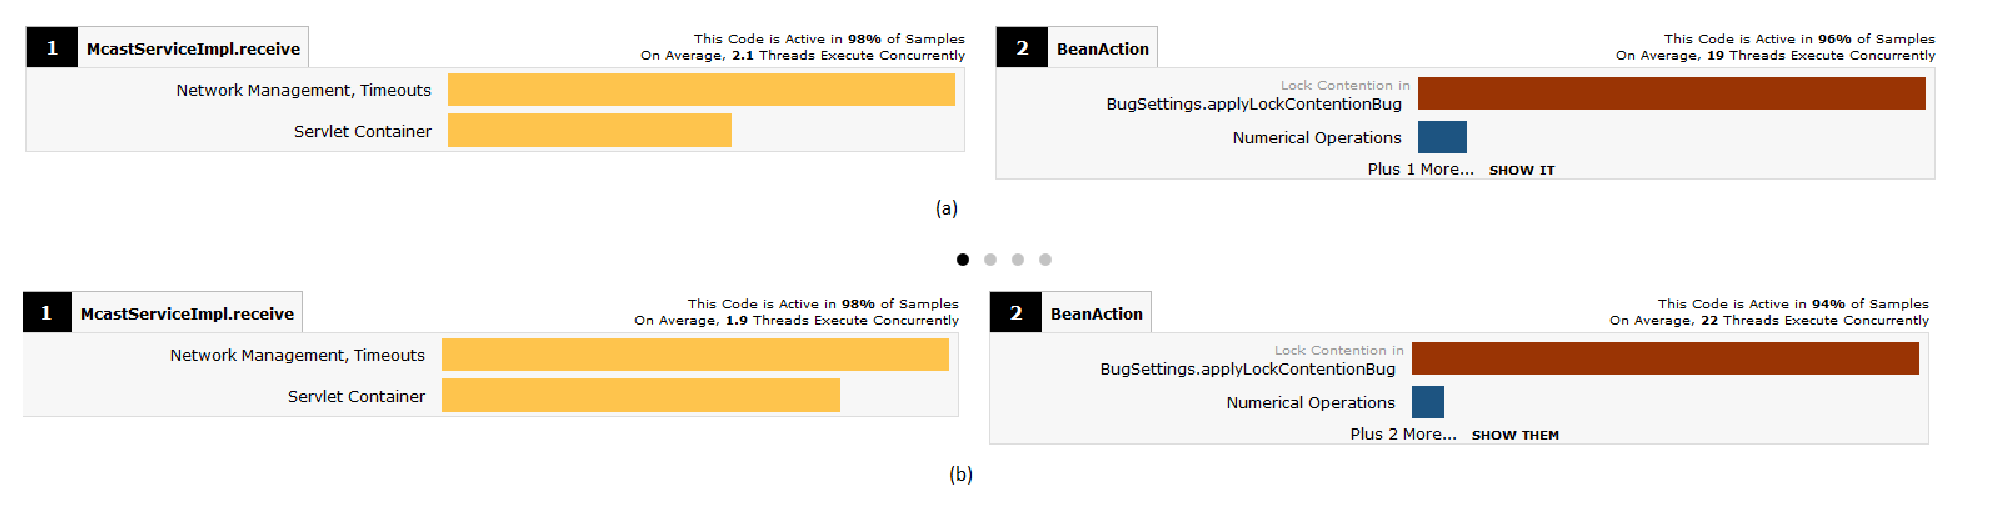
\includegraphics[totalheight=.22\textheight,width=1\textwidth]{run1_issues12_short_long_run}
\caption{Top detected performance issues in modified JPetStore application}
\label{fig_run1_bugs12}
\end{figure}

After identifying an issue, a tester can see more details, including the type of
problem, involved class, method and method line. \figurename
~\ref{fig_issue2_vs_code} shows the information of our Lock Contention bug,
which was located in the LockContentionBug class, the method generateBug and the
line 20. When comparing this information with the actual code, one can see that
is precisely the line where the bug was injected (taking a class lock before
doing a very CPU intensive logic).
\vspace{-5pt}
\begin{figure}[!h]
\centering
\includegraphics[totalheight=.22\textheight,width=1\textwidth]{issue2_vs_code}
\caption{Lock contention issue in the WAIT report and the actual source code}
\label{fig_issue2_vs_code}
\end{figure}
\vspace{-5pt}
In 3rd place the report showed a symptom of the lock contention issue
(the issues were correlated by comparing their detail information, which
pinpointed to the same class/method), suggesting this was a major issue. The I/O
latency bug was identified in 4th place. \figurename ~\ref{fig_issues34} shows
the details of these issues.

\begin{figure}[!h]
\centering
\includegraphics[totalheight=.23\textheight,width=1\textwidth]{run1_issues34_details}
\caption{Details of issues ranked 3 and 4 in the first test run}
\label{fig_issues34}
\end{figure}

The deadlock issue did not appear in this first run, somehow prevented by the
lock contention bug which had a major impact that planned. As in any common
test phase, the identified bugs were ``fixed'' and a new run was done to review
if any remaining performance issues existed. Not surprisingly, the deadlock bug
appeared. \figurename ~\ref{fig_dlissue_vs_code} shows the information of our
Deadlock bug, which was located in the line 30 of the DeadLockBug class. This is
precisely the line where the bug was injected (as the deadlock occurs when the
friends bow back to each other).
\vspace{-5pt}
\begin{figure}[!h]
\centering
\includegraphics[totalheight=.23\textheight,width=1\textwidth]{deadlock_vs_code}
\caption{Deadlock issue in the WAIT report and the
actual source code}
\label{fig_dlissue_vs_code}
\end{figure}
\vspace{-5pt}

This experiment was considered successful as all injected bugs were identified,
including the involved classes and methods. In terms of time, two main savings
were documented. First, the automated approach practically reduced the effort of
collecting data for WAIT to zero. After a one-time installation which took no
more than 15 minutes for all nodes, no time was spent using the automate
approach, only requiring a few seconds to modify its  configuration
whenever needed(i.e. to change the \emph{Sampling Interval}). The second time
saving was in the analysis of the WAIT reports. Previously, a tester would have
ended with multiple reports. Now a tester only needs to monitor a single report
which gets refreshed periodically.

Overcoming the usability constraints of WAIT also allow a tester to exploit
WAIT's expert knowledge capabilities. Even though it might be hard to define an
average time spent identifying performance issues, a conservative estimate (i.e.
2 hours) could help to quantify WAIT's savings. In our study case, instead of
spending an estimate of 6 hours analyzing the issues, it was possible to
identify them and their root causes with the information provided by the WAIT
report. As seen in the experiment, additional time can also be saved by
reporting relevant issues in parallel to the execution of the test. This is
especially valuable in long-term runs, common in performance testing, and which
usually last several days.

In conclusion, the results of this second experiment answered our research
question Q3 (What benefits in productivity can a tester achieve if the previous
two questions are answered?), showing the productivity gains that a tester
achieves by using the automated approach of WAIT.

To summarize the experimental results, they were satisfactory because it
was possible to achieve the goal of automating the execution of WAIT,
while keeping the overhead low (in the range of 0\% to 3\% using a \emph{Sample
Interval} of 480 seconds). Besides the automated approach brought several time
savings to a tester: After a quick installation (around 5 minutes per node), the
time required to use an automated WAIT was practically zero. A tester now only
needs to monitor a single WAIT report, which offers an incremental view of the
results. A direct result of these savings is the reduction in effort and expert
knowledge required by tester to identify performance issues, hence improving the
productivity.

\vspace{-5pt}
\subsection{Threads to Validity}
\vspace{-5pt}
Like any empirical work, there are some threats to the validity of these
experiments. First the possible environmental noise that could affect the test
environments because they are not isolated. To mitigate this, multiple runs were
executed for each identified combination. Another thread was the selection of
the tested applications. Despite being real-world applications, their limited
number implies that not all types of applications have been tested and wider
experiments are needed to get more general conclusions. However, there is no
reason to believe that the approach is not applicable to other environments.

%%%%%%%%%%%%%%%%%%%%%%%%%%%%%%%%%%%%%%%%%%%%%%%%%%%%%%%%%%%%%%%%%%%%%%%%%%%%%%%%%%%%%%%%%%%%%%%%%%%%%%%%%%%%
% Section 7: Conclusions
%%%%%%%%%%%%%%%%%%%%%%%%%%%%%%%%%%%%%%%%%%%%%%%%%%%%%%%%%%%%%%%%%%%%%%%%%%%%%%%%%%%%%%%%%%%%%%%%%%%%%%%%%%%%
\vspace{-5pt}
\section{Conclusions and Future Work}
\vspace{-5pt}
The identification of performance problems and the diagnosis of their root
causes in highly distributed environments are complex and time-consuming tasks,
which tend to rely on the expertise of the involved engineers. The objective of
this work was to address the limitations that prevented the usage of WAIT in
performance testing, so that it can be effective used to reduce the expertise
and effort required to identify performance issues and their root causes. To
achieve this goal the paper presented a novel automation approach and its
validation, composed of a prototype and study cases with two real-life
applications. The results are encouraging as they have proved that the approach
addresses effectively the adoption barriers of WAIT in performance testing: The
solution has proven light-weight, generating low overhead (in the range of 0\%
to 3\% using a \emph{Sample Interval} commonly used in the industry). Moreover,
there are also tangible time savings in terms of the effort required to detect
performance issues.

Future work will concentrate on assessing the approach and its benefits through
broader study cases with our industrial partner IBM with a special interest in
understanding the trade-off between the \emph{Sampling Interval} and the nature
of the applications (represented by their \emph{Javacores}). It will also be
investigated how best to exploit the functional information that can now be
obtained from a tested environment (i.e. workload, throughput or transactions)
to improve the qualitative and quantitative capabilities of the idle-time
analysis to identify more types of performance problems.

%%%%%%%%%%%%%%%%%%%%%%%%%%%%%%%%%%%%%%%%%%%%%%%%%%%%%%%%%%%%%%%%%%%%%%%%%%%%%%%%%%%%%%%%%%%%%%%%%%%%%%%%%%%%
% Section 8: Acknowledgements
%%%%%%%%%%%%%%%%%%%%%%%%%%%%%%%%%%%%%%%%%%%%%%%%%%%%%%%%%%%%%%%%%%%%%%%%%%%%%%%%%%%%%%%%%%%%%%%%%%%%%%%%%%%%
\vspace{-5pt}
\section*{Acknowledgments}
\vspace{-5pt}
We would like to thanks Amarendra Darisa, from SVT IBM, as his experience in
performance testing helped us through the scope definition and validation. This
work was supported, in part, by Science Foundation Ireland grant 10/CE/I1855 to Lero - the Irish Software Engineering Research Centre (www.lero.ie).

% Between 12 - 24 \ldots 18 sounds like a good number!
\bibliographystyle{splncs}
\bibliography{dwait_manual,dwait}

%\section*{Appendix: Springer-Author Discount}

\end{document}

----------------------------
  
PENDING:
- Re-read the paper to see if it makes sense (i.e. the verbiage of the reserch
questions should change to make a better fit with the experiments and their results).

[STANDBY: Should I add any mention of the sanity check? (about HD) probably
only if suggested]

[STANDBY: Should I bring back the pseudo-motivation of expert -maybe
automation efforts to reduce the expert knowledge required to do performance
testing/analysis:  (i.e. RTCE, GC Lite, LeakChaser), runtime vs. static. Some
similar, but different in the sources they use and the domain?-]

------------

Bg:

This can be caused by multiple factors,
such as resource constraints, locking problems or excessive system-level activities.

This characteristic is especially relevant considering that the JVM has to pause its running applications whenever a
\emph{javacore} is generated. Even though a JVM can produce \emph{javacores}
with a fairly low perturbation, these pauses might go up to several hundred
milliseconds if the application has thousands of concurrent threads and very
deep call stack traces. 

Related Work:

- Automation:

Load Testing: Avritzer1, Avritzer2

A similar trend occurs in the industry, where exist multiple products for
this task. For example, the HP LoadRunner \footnote{http://www8.hp.com/us/en/software/ software-product.html?compURI=tcm:245-935779} and the IBM's Rational Performance
Tester \footnote{http://www-01.ibm.com/software/awdtools/tester/performance/}
are commercial solutions that allow scalability testing by generating real
workloads on the application, while Apache's JMeter
\footnote{http://jmeter.apache.org/} is the most popular open-source choice.

- Performance Analysis:

Chun1
The goal of the work is to
develop and evaluate tools for offline and online analysis
of system metrics gathered from instrumentation in Internet
server platforms. We use a promising class of probabilistic
models (Tree-Augmented Bayesian Networks or
TANs) to identify combinations of system-level metrics
and threshold values that correlate with high-level performance
states—compliance with Service Level Objectives
(SLOs) for average-case response time—in a threetier
Web service under a variety of conditions.
Experimental results from a testbed show that TAN
models involving small subsets of metrics capture patterns
of performance behavior in a way that is accurate
and yields insights into the causes of observed performance
effects. TANs are extremely efficient to represent
and evaluate, and they have interpretability properties
that make them excellent candidates for automated diagnosis
and control. We explore the use of TAN models for
offline forensic diagnosis, and in a limited online setting
for performance forecasting with stable workloads.

Agarwala1
The work by Aguilera et al. [1] is most closely related
to E2Eprof. They propose two algorithms to determine
causally dependent paths and the associated delays from
the message-level traces in a distributed system. While
their nesting algorithm assumes ‘RPC-style’ (call-returns)
communication, their convolution algorithm is more general
and does not assume a particular messaging protocol.
Our pathmap algorithm is similar to the convolution algorithm,
in that both uses time series analysis and can handle
non-RPC-style messages. While the convolution algorithm
is primarily intended for offline analysis, pathmap
uses compact trace representations and a series of optimizations,
which jointly, make it suitable for online performance.


Problem Statement:

An possible assumption that can be considered to use WAIT in its current form
in a performance test is that the different JVMs that composed a
distributed environment usually face the similar type of performance
bottlenecks, so the analysis can focus on a single randomly selected JVM and it
can be assumed that its results are representative of the whole system. Even
though this assumption might be applicable in other scenarios, it does not suit
performance testing because performance testing is responsible of assuring that
the application will be able to handle the planned workload in production. If a
single node is assessed, there is a high risk that other potential issues are
been overlooked. The probability of the risk would be directly related to the
size of the distributed system  (the bigger the number of nodes, the most
likely a single node is not representative) and the type of performance tests
been developed (it is common that different random factors and request
distributions are used to emulate diversity in the behavior of the users,
which usually involve that different nodes process different types of
transactions at different rates).

Approach / Implementation:

Approach:
Even though the above approach has been defined to address the usability needs
of WAIT, it should be noted that its structure is flexible enough to be easily
adjusted to fit automation scenarios of similar characteristics.

Arch:
Internally, it reuses the data gathering scripts that are currently available for WAIT
\footnote{https://wait.ibm.com/\#page=dataCollectors}. 

Arch/Proto:

Two key assumptions were taken when defining this design. As the scope of this
work is the performance testing, it is assumed that a Load Testing tool will always be
present. Moreover this work has focused on Web Applications, so it is assumed
that there will be a Web Application Server in each application node. This
assumption allows the \emph{WAIT Node Agent} to be a Web Application.
As it uses plain HTTP request to interact with the \emph{WAIT Control Agent}, a
single version of \emph{WAIT Node Agent} could easily interact with multiple
types of \emph{WAIT Control Agent} (as it will be very likely to have one per
type of Load Testing Tool) or even used independently.


Experiments:

Experiment 1:

Test 1:
, which directly calculates throughput and response
time, while it obtained the resources' utilization from the Windows Performance Monitor
\footnote{http://technet.microsoft.com/en-us/library/cc768048.aspx} of each application node.

Unlike Sun’s, JPetStore is a reimplementation with a more efficient design
\footnote{www.clintonbegin.com/downloads/JPetStore-1-2-0.pdf‎}. 
\footnote{http://tomcat.apache.org/}
application which offers enterprise portal capabilities and which is, as per
Gartner Research comparison of software for horizontal portals, 
\footnote{http://www-01.ibm.com/software/webservers/appserv/was/}.

Each one performed in an unloaded single-node environment, with the
corresponding Application Server restarted before every run.

, with 99\% of successful transactions

Test 2:
due to the available of an environment to test it as well as the availability of
its source code (required for the experiment \#2)

, with 99\% of successful transactions

Experiment 2:

Similarly to the previous cases, the report information, complemented
with its comparison against the source code allowed the issue identification.
A point worth noticing is that, even though the presence of the issue was
correctly identified by WAIT, in this particular case it was not able to
categorize it (leaving it with a blank color).

The automated approach would allow a wider range of testers to do performance
analysis. An additional benefit is that less experienced testers could use this
information to gain a deeper understanding of these type of problems, hence
reducing the dependency and overall workload of the most expert users within a team.

%\footnote{https://wait.ibm.com/waitUserManual.pdf}

As the measurement of success for this experiment was to the ability of WAIT to
identify performance problems, 

Assuming an environment composed of X nodes, with a desired time window of
1-hour and a test duration of Y hours, a tester would have ended with X*Y different WAIT reports, 
having to review X reports per hour. 

In summary \ldots
Previously the number of WAIT reports a tester needed to review was equal to the
number of nodes multiplied by the times the collected data was uploaded; 


Threads to Validity:

Also to determine if the differences in the results were statistically
significant (with 90\% of certainty), Paired t-Tests were applied.


Another thread was the selection of the test parameters (i.e. workload and
duration). This was addressed with the expert judgement of the SVT, which guided
on their selection. Finally, the validity of the results are threatened by the
selection of the tested applications. 